\section{{\name} Implementation}
\label{sec:system}

%\subsection{System Design}

% \desc{Why do people need Allox?}

% In existing resource managers such as Kubernetes, a job submitted in one configuration cannot be executed on other sources.
%To the best of our knowledge, \name is the first resource allocation system allowing multiple job configurations.
We build \name based on Kubernetes using roughly 3000 lines of Go code for the resource manager and 1500 lines of Python for its online job estimation tool.
We pick Kubernetes because it well supports clusters consisted of heterogeneous resources such as CPU and GPU.

\name has three main components: \emph{Estimator}, \emph{Scheduler}, and \emph{Placer}.
\name first uses the estimator to obtain job characteristics.% of machine learning jobs.% is implemented as in (\S\ref{sec:res_estimation}). 
%The configurations and speed-up rates are fed as input to Scheduler.
The scheduler then uses the algorithm described in the previous section to decide which job to be scheduled next and whether to place it on CPU or GPU.
%The scheduler then decides which jobs to be executed.
Finally, the placer executes the schedule in the system. %the scheduled jobs on the right resource (CPU or GPU). 
The \name system is depicted in Figure \ref{fig:design}.

%\paragraph{Multi-resource Manager}
\begin{figure}
	\centering
	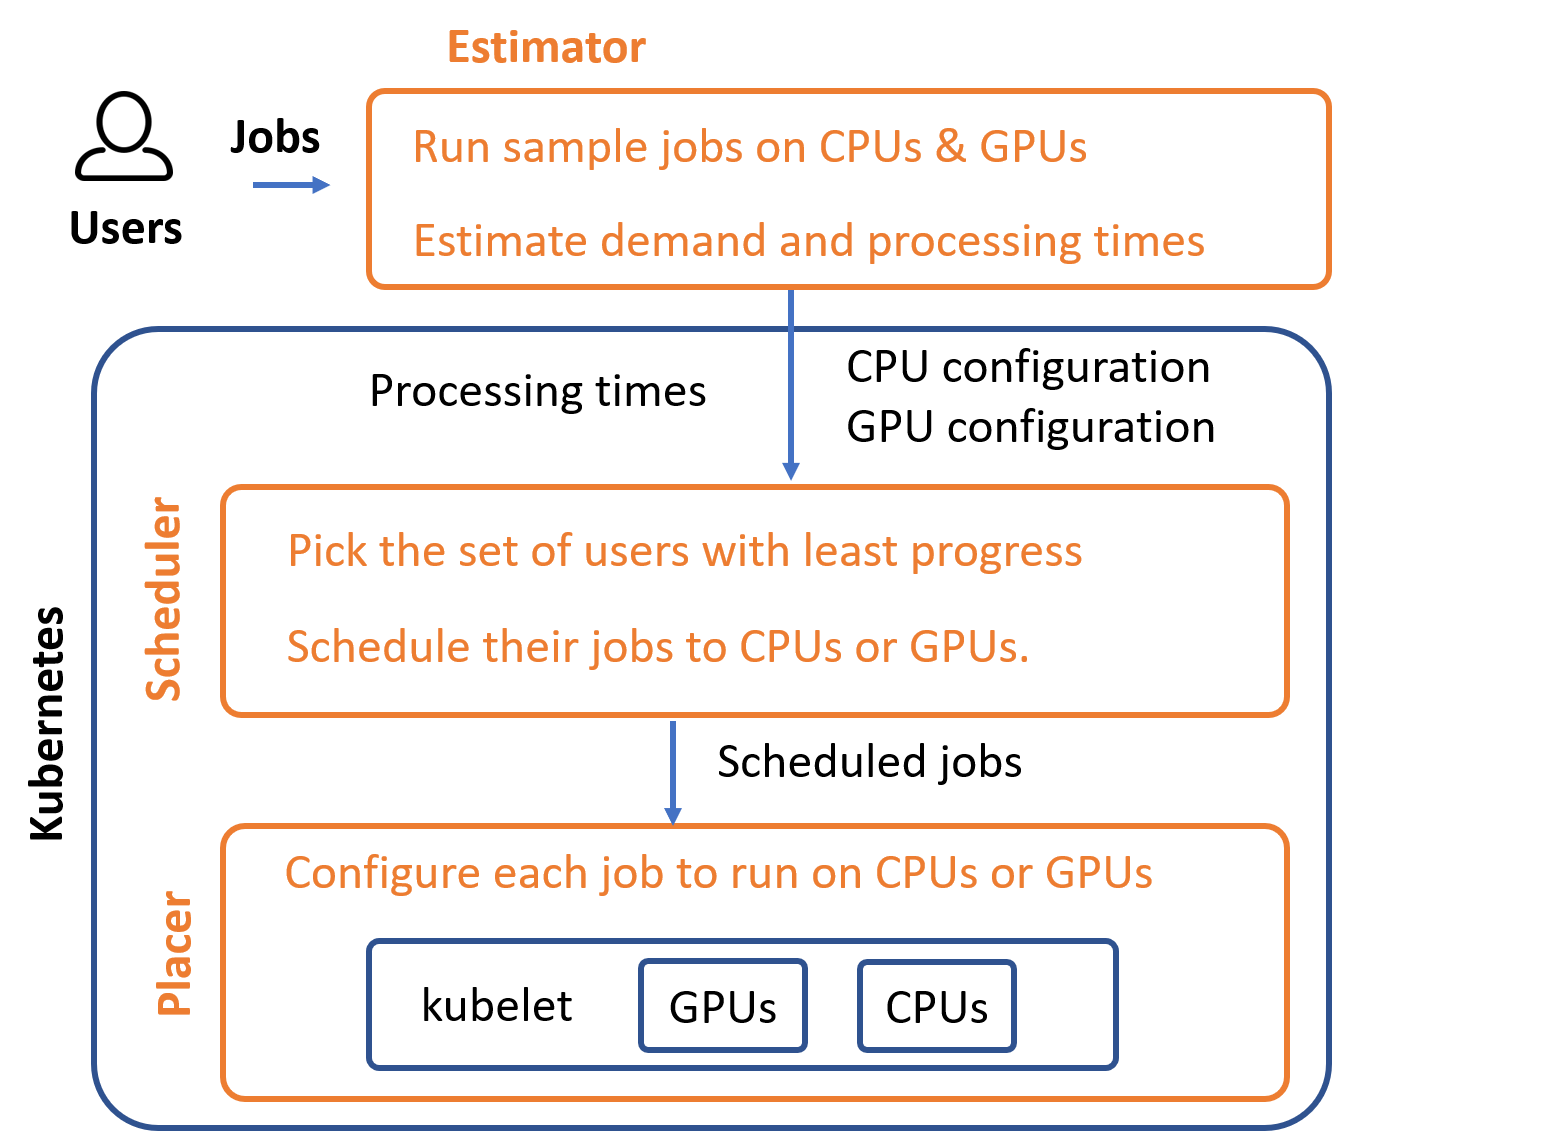
\includegraphics[width=1.0\linewidth]{figs/design}
	\caption{The \name system has three main components: Estimator, Scheduler, and Placer.}
	\label{fig:design}
\end{figure}

\subsection{Estimator}\label{sec:profiling}
%\emph{Estimation Tool}. 
The estimator predicts jobs' resource demands and their processing times on CPU and GPU in an online manner. %to provide information necessary for the schedule to make decisions.
%Users use to submit their jobs via the estimation tool.
For each job, it creates four samples of the job -- two for CPU and the others for GPU -- that are much smaller than the original job.
In our experiment, the total length of the sample jobs is 3\% of the real jobs. While the real jobs can run for hours, the samples last from 30 seconds to 2 minutes. 
Based on the completion time of the samples, we estimate the processing time of the real job on both CPU and GPU. The estimation is relatively accuracy, especially for most machine learning jobs that are iterative~\cite{ernest, slaq_socc17}. 
Figure~\ref{fig:prediction_errors_cdf} shows the CDF of estimation errors of 40 jobs through real experiments. The mean absolute error is 8\% and the standard deviation is 11\%. 

\begin{figure}[h]
	\centering
	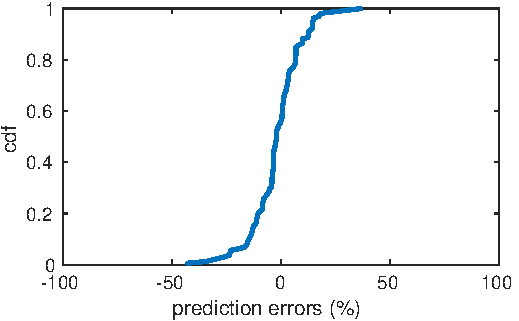
\includegraphics[width=0.7\linewidth]{figs/prediction_errors_cdf}
	\caption{CDF of the estimation errors from experiments.}
	\label{fig:prediction_errors_cdf}
\end{figure}


% Figure \ref{fig:est_compl_time} shows that the completion time of TensorFlow benchmark jobs on GPU are proportional to number of batches.
% \begin{figure}[h]
%   \centering
%   %    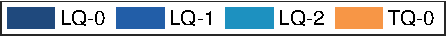
\includegraphics[width=0.6\linewidth]{fig/b1i3_res_usage_legend}
%   {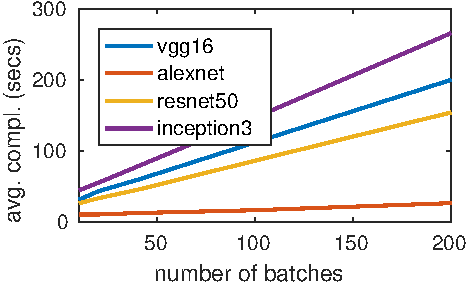
\includegraphics[width=0.7\linewidth]{figs/prof-batchnum-gpu} \label{fig:prof-batchnum-gpu}}    \hspace{0.0in}
%   \caption{(a) The completion times of jobs linearly increase with respect to number of batches.}
%   \label{fig:est_compl_time}
% \end{figure}

%The estimation tool estimates the job completion time using a pair of samples.
%Each sample is a scale version of the job.


% \begin{figure}[!h]
%   \centering
%   \subfloat[] {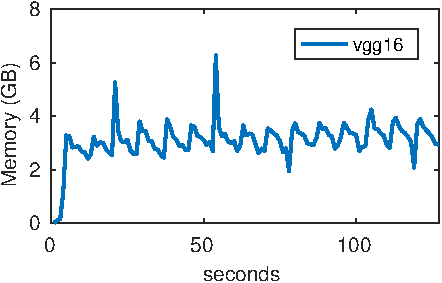
\includegraphics[width=0.45\linewidth]{figs/mem_usage_logcpu} \label{fig:mem_usage_logcpu}}    \hspace{0.1in}
%   \subfloat[] {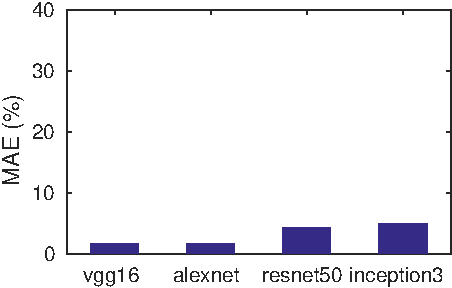
\includegraphics[width=0.45\linewidth]{figs/mem_usage_errcpu} \label{fig:mem_usage_errcpu}}
%   \caption{(a) The memory usage of an ML job has a similar pattern overtime (b) Averaging the memory usage of the short versions can estimate the memory usage average of the job at high accuracy.}
%   \label{fig:mem_usage}
% \end{figure}

% \desc{picking memory}

Similar to Gandiva \cite{gandiva_osdi18}, the estimator determines the memory demands of jobs by monitoring the memory usage of their corresponding samples. 
% As shown in Figure~\ref{fig:mem_usage}, using the sample can predict job's memory demand with acceptable accuracy.

% \desc{picking GPU}

Currently, GPUs do not support fine-grain sharing among multiple jobs \cite{gandiva_osdi18}.
Therefore, a job needs to use a whole GPU in \name. %, a GPU is not shared by multiple jobs in \name, and a job's GPU configuration needs an integral number of GPUs. 
% normally needs a whole GPU.
%A GPU is often powerful enough to carry an ML job.
%If a ML job is paralleled on multiple GPUs, we can consider it as multiple independent jobs.

%Although GPU memory can be statically shared but this results in worse performance due to memory contention.
%Furthermore, GPU memory is limited so ML jobs prefer to fully utilize the GPU memory for their performance.
%ML job and multiple GPUs are not performance effective when they do not support peer-to-peer transfers.
% \desc{picking CPU}
For CPU, the estimator picks the maximum number of cores in a CPU to optimize the performance of the job on CPU.
% Figure \ref{fig:cpu_cores} shows that the performance of TensorFlow jobs is much better using more CPU cores.
As Kubernetes does not allow a container to have more than 1 CPU, \name does not give more CPU cores than a single physical CPU has.
% \begin{figure}[!h]
%   \centering
%   \subfloat[vs. a single CPU core] {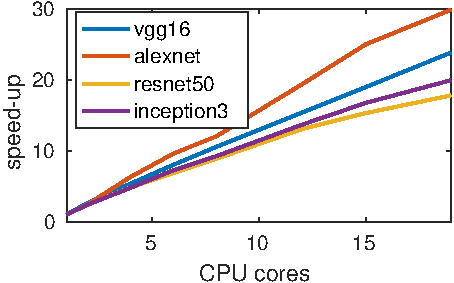
\includegraphics[width=0.7\linewidth]{figs/prof_cpu_speedup} \label{fig:prof_cpu_speedup}}    \hspace{0.1in}
%   %     \subfloat[] {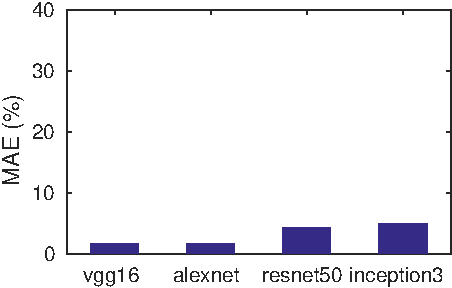
\includegraphics[width=0.45\linewidth]{figs/mem_usage_errcpu} \label{fig:mem_usage_errcpu}}
%   \caption{Users prefer to use more CPU cores as using them significantly improve jobs v.s. using a core.}
%   \label{fig:cpu_cores}
% \end{figure}


\subsection{Scheduler}
%\desc{Scheduler}
%We enable fair resource allocation and job scheduling on Kubernetes scheduler.
Kubernetes does not support fair allocation or job scheduling. As a result, we cannot simply modify some existing scheduler for our algorithm. 
%Given the allocation and CPU/GPU configurations,
%the scheduler chooses which jobs to be scheduled on CPU or GPU.
Instead, we implement our scheduler from scratch using the \textit{kube-scheduler} API.



%The scheduler is mainly implemented by customizing in \textit{kube-scheduler}.
%Although we borrow some fundamental APIs from \textit{kube-scheduler}, several features are significantly changed.

% We add job scheduling in \textit{kube-scheduler}.
% There is a single queue for all available jobs (a.k.a. pods).
% Allocating resources to a pod may take a few seconds in the distributed systems.
% If there are many pods queued up, waiting time in the queue can be large. 
% To allocate resources the pods quickly, \textit{kube-scheduler} schedules pods in an asynchronous manner.
% The scheduler keeps popping pods out of the queue whenever a new pod arrives.
% If a pod is not successfully admitted, it will be added to the queue.
% Basically, the queue has maximum one element at any time.
% However the scheduler requires multiple jobs in the queue so that they pick the best one.
%\todo{Tan, add what you changed \textit{kube-scheduler} to implement the scheduler. DONE} 
Jobs arrive in a single queue in \textit{kube-scheduler}.
Given the set of available jobs, the scheduler decides which job to run. 
\textit{kube-scheduler} receives the estimated processing times of the CPU and GPU configurations from the estimator and passes them to \name scheduler via \textit{kubectl}. 
\name scheduling procedure is activated prior to \textit{Pod Admission}.
%\textit{Pod Admission} then forwards the job to an appropriate node.
If the job is not admitted, it is sent back to the waiting queue.
% The job is picked such that it minimizes the average completion time maintain fairness among users as we present in \S~\ref{sec:alg}.
In addition to our scheduling algorithm, we implement other methods described in Section~\ref{sec:baselines}.

We add fairness support to \textit{kube-scheduler} by updating the progress of all users over time \S~\ref{sec:fairness_score}.
\textit{schedulerCache} in \textit{kube-scheduler} captures the snapshot of the whole system.
When there is an update from the system, \textit{schedulerCache} is notified and \name checks if a job gets resources or finishes.
If a job receives allocated resources, the progress of that user is increased accordingly.
Recall that if a job is running with the unfavorable configuration (with longer processing time), the progress increase is discounted.% from the that of running on the favorable configuration. 
If a job finishes, we deduct its progress from the corresponding user.

%\todo{Tan, add what you changed \textit{kube-scheduler} for fairness.  -- DONE} 

%The key idea of \textit{kube-scheduler} is to fit the pods into available resources in the FIFO manner without considering user resource usage.
%In our scheduler, there are multiple users and a user is mapped to a \textit{namespace} in \textit{kube-scheduler}.
%As a job can be allocated in either on CPU or GPU, fairness cannot rely on resource usage.
%We have our fairness score that actually can generalize the resource usage fairness.


\subsection{Placer}
The placer \emph{dynamically} configures proper containers and executes jobs within these containers.
In the current Kubernetes system, jobs are configured to run on CPU or GPU ahead of time; hence, they do not need the placer.
This is another new component added.% to the current Kubernetes system.

\subsection{Operational issues}

\paragraph{Minimum CPU Per Job}
When developing our scheduler, we realized all jobs running on GPUs also require (a small amount of) CPU for proper execution.
\name addresses this by reserving a small number (one by default) of CPU cores for GPU jobs.%; e.g., we can reserve 1 CPU cores for each GPU.
As the number of CPU cores in a cluster is often large, this change has little impacts on the performance.

\paragraph{Job profiling overhead}
Before a job is scheduled, its sample jobs must be completed first. 
To this end, \name prioritizes all sample jobs. 
Because these sample jobs are relatively small, the overhead is minimal.  
\name also sets a limit on resources for sample jobs to reserve enough resources for the real jobs. In addition, if a sample job is significantly longer than others, we do not need to complete it as it already indicates the original job is very long. We can adjust the sample job size to balance the overheads and estimation accuracy.

\paragraph{Low utilization with small $\alpha$ }
The fairness parameter, $\alpha$, allows the explicit tradeoff between fairness and performance.
However, when $\alpha$ is small, the small set of users may not have jobs or want to wait for better resources, e.g., there are available CPUs but they prefer to wait for GPUs.
%However, these users may not want to execute their jobs on the available machines.
This results in low resource utilization.
To deal with this, \name temporally increases $\alpha$ to include more users who need the available resources.
%If resources (CPUs or GPUs) are still available, we do this until all users are considered, i.e., $\alpha \geq 1$.

\paragraph{Resource availability}
%\name relies on estimated completion times to know when a node will become available, which is needed for the scheduling algorithm.
While it is sufficient to use estimated processing times in the scheduling algorithm, resource availability needs to be obtained separately over time because there may be significant estimation errors. 
%Since there are estimation errors, the availability times are not the same as expected.
%In this case, \name needs to know the availability of machines. 
By default, Kubernetes periodically checks the health and updates from each node. Therefore, resource availability can be collected together with the current health check without additional overheads. %the events if the nodes are healthy and updates the (\textit{schedulercache.NodeInfo}).
If we need to inquire the availability information from all nodes very frequently, it might still lead to significant communication overheads for large-scale clusters. In this case, the information of nodes and jobs (\textit{schedulercache.NodeInfo}) are cached in each node and can be updated via events to the master node. 
%Therefore, Kubernetes can periodically checks the events if the nodes are healthy and updates the (\textit{schedulercache.NodeInfo}).
%Meaning, \name can obtain the node availability via \textit{schedulercache.NodeInfo} without creating additional overheads.

%If a job finishes before its expected completion time, we update the corresponding resources' availability.
%If it finishes after, we do not schedule any new jobs on the resources occupied by that job.

\paragraph{Scalability}
The network flow problem for job scheduling can be solved in polynomial time. Using the Hungarian algorithm, the computation complexity is $\mathcal{O}((mn)^3)$ where $m$ is the number of nodes and $n$ is the number of jobs. In a large-scale system with many jobs to schedule simultaneously, this might become the bottleneck.
%\name can be computationally bottlenecked in solving the matching problem for scheduling.
To reduce the complexity, \name picks a subset of jobs instead of the entire queued up jobs based on the processing time on each resource, and it still provides similar performance but with much fast speed. This is validated in Section~\ref{sec:N_max}.
%We limit $N_{max}$, the maximum size of the subset.
%We pick up to $N_{max}$ jobs such that they are either shortest on CPU or GPU.
%Intuitively, \name prefer to schedule the short jobs first.
%We show that small $N_{max}$ still achieves a very close performance to the optimal one in \S\ref{sec:N_max}.